\documentclass[a4paper,twoside,12pt]{article}
\usepackage{amsmath}
\usepackage{amsfonts}
\usepackage{amssymb}
\usepackage[utf8]{inputenc}
\usepackage[T1]{fontenc}
\usepackage{fancyhdr}
\usepackage{stmaryrd}
\usepackage{textcomp}
\usepackage[french]{babel}
\usepackage{variations}
\usepackage{graphicx}
\usepackage{array}
\usepackage{arydshln}
\usepackage{verbatim}
\usepackage{psfrag}
\usepackage{bbm}
\usepackage{ifthen}

\newlength{\myhoffset}
\newlength{\mytextwidth}
\newlength{\myvoffset}
\newlength{\mytextheight}
\setlength{\myhoffset}{-1cm}
\setlength{\mytextwidth}{2.5cm}
\setlength{\myvoffset}{-2.5cm}
\setlength{\mytextheight}{3cm}

\addtolength{\hoffset}{\myhoffset}
\addtolength{\textwidth}{\mytextwidth} 
\addtolength{\voffset}{\myvoffset}
\addtolength{\textheight}{\mytextheight} 

%textpos : permet de placer des éléments par leur coordonnées absolues sur la page
% utilisé pour les entêtes et pied de pages

\usepackage[absolute]{textpos}
\setlength{\TPHorizModule}{1mm}
\setlength{\TPVertModule}{\TPHorizModule}
\textblockorigin{-\myhoffset}{-\myvoffset}

% appendix : permet d'écrire en couleur

\usepackage[usenames,dvipsnames]{xcolor}

% fancyhdr : permet de personnaliser les entêtes et pieds de page des documents

\usepackage{fancyhdr}

%% pdfpages : utilisé pour insérer la page de garde avant le document

\usepackage{pdfpages}

% caption : centre les légendes des figures

\usepackage[center]{caption}

% wrapfig : permet de créer des figures entourées de texte

\usepackage{wrapfig}

%placeins : permet d'obliger Latex à insérer les figures en attente avant de continuer

\usepackage{placeins}

% subfig : permet de créer des figures avec plusieurs sous-figures

\usepackage{subfig}

% appendix : permet de gérer les annexes

\usepackage[page]{appendix}

\setlength\parindent{0pt}

\linespread{1.1}


%%%% debut macro %%%%
\makeatletter
\def\hlinewd#1{%
\noalign{\ifnum0=`}\fi\hrule \@height #1 %
\futurelet\reserved@a\@xhline}
\makeatother
%%%% fin macro %%%%

\newcounter{partie}
\newcounter{sous-partie}

\renewcommand{\thesection}{\Roman{section}}

\newenvironment{partie}[1]
{
\section{#1}
}
{

}

\newcommand{\mymark}[1]{\markboth{\MakeUppercase{#1}}{\MakeUppercase{#1}}}

\newenvironment{biblio}
{
\section*{Bibliographie}
\addcontentsline{toc}{section}{Bibliographie}
\mymark{Bibliographie}
}
{

}

\newenvironment{intro}
{
\section*{Introduction}
\addcontentsline{toc}{section}{Introduction}
\mymark{Introduction}
}
{

}

\newenvironment{remerciements}
{
\section*{Remerciements}
\addcontentsline{toc}{section}{Remerciements}
\mymark{Remerciements}
}
{

}


\newenvironment{sous-partie}[1]
{
\subsection{#1}
}
{

}

\newenvironment{sous-sous-partie}[1]
{
\subsubsection{#1}
}
{

}

\newenvironment{liste}
{
\vspace{0.2cm}
\begin{list}{$\bullet$\hspace{0.3cm}}{\leftmargin=1.4cm}
}
{
\end{list}
\vspace{0.2cm}
}

\newcounter{numannexe}
\newenvironment{annexes}
{
\newpage
\thispagestyle{empty}
\mbox{}
\newpage
\addcontentsline{toc}{section}{Annexes}
\mymark{Annexes}
\vspace*{\fill}
\begin{center}
\Huge{\textbf{Annexes}}
\end{center}
\vspace*{\fill}
\newpage
\setcounter{numannexe}{1}
}
{

}

\newenvironment{annexe}[1]
{
\addcontentsline{toc}{subsection}{Annexe \arabic{numannexe} : #1}
\mymark{Annexe \arabic{numannexe} : #1}
\subsection*{Annexe \arabic{numannexe} : #1}
\stepcounter{numannexe}
}
{
}

\newenvironment{sous-annexe}[1]
{
\begin{subappendices}
\subsection{#1}
}
{
\end{subappendices}
}


% Divers

% Permet de faire des cadres dans le document
\newcommand{\cadre}[1]{\renewcommand{\arraystretch}{0.4}\begin{array}{|c|}\hline\\#1\\\\\hline\end{array}}
\newcommand{\cadret}[1]{\renewcommand{\arraystretch}{0.4}\begin{tabular}{|c|}\hline\\#1\\\\\hline\end{tabular}}
\newcommand{\semicadre}[1]{\renewcommand{\arraystretch}{0.3}\begin{array}{c|}#1\\\\\hline\end{array}}

% Commandes mathématiques

\newcommand{\equivalent}[2]{\!\!\renewcommand{\arraystretch}{1}\begin{array}[t]{c}\Huge\sim\\^{#1\rightarrow#2}\end{array}\!\!}
\newcommand{\tend}[2]{\!\renewcommand{\arraystretch}{1}\begin{array}[t]{c}-\!-\!\!\!\longrightarrow\\^{#1\rightarrow#2} \\ [-1.5ex]\end{array}\!}
\newcommand{\egal}[2]{\!\!\renewcommand{\arraystretch}{1}\begin{array}[t]{c}=\\^{#1\rightarrow#2}\end{array}\!\!}
\newcommand{\fin}{\vspace{0.2cm}\\}
\newcommand{\finq}{\vspace{0.5cm}\\}
\newcommand{\sh}{\mathrm{sh}\,}
\newcommand{\abs}[1]{\left\vert#1\right\vert }
\newcommand{\ch}{\mathrm{ch}\,}

\renewcommand{\o}[1]{\mathrm{o}\!\left(#1\right)}
\newcommand{\etoile}{\hspace*{1cm}$\star$\hspace*{0.5cm}}
\renewcommand{\th}{\mathrm{th}\,}
\renewcommand{\arcsin}{\mathrm{Arcsin}\,}
\renewcommand{\arccos}{\mathrm{Arccos}\,}
\newcommand{\argsh}{\mathrm{Argsh}\,}
\newcommand{\argch}{\mathrm{Argch}\,}
\newcommand{\argth}{\mathrm{Argth}\,}
\newcommand{\rg}{\mathrm{rg}\,}
\renewcommand{\arctan}{\mathrm{Arctan}\,}
\newcommand{\sq}{\hspace*{1.4cm}\stepcounter{sq}(\alph{sq})\hspace*{0.5cm}}
\newcommand{\rcl}{\begin{array}{rcl}}
\newcommand{\ea}{\end{array}}
\newcommand{\str}[1]{\renewcommand{\arraystretch}{#1}}
\renewcommand{\tfrac}[2]{\textstyle\frac{#1}{#2}}
\newcommand{\Cl}[1]{$C^{#1}$}
\newcommand{\mathCl}[1]{C^{#1}}
\renewcommand{\t}[1]{\tilde{#1}}
\renewcommand{\l}{\lambda}
\newcommand{\ds}{\displaystyle}
\newcommand{\R}{\mathbb{R}}
\newcommand{\C}{\mathbb{C}}
\newcommand{\Q}{\mathbb{Q}}
\newcommand{\Z}{\mathbb{Z}}
\newcommand{\N}{\mathbb{N}}
\newcommand{\Ker}{\mathrm{Ker}\,}
\newcommand{\Vect}{\mathrm{Vect}}
\renewcommand{\lvert}{\left\vert}
\renewcommand{\Im}{\mathrm{Im}\,}
\renewcommand{\rvert}{\right\vert}
\newcommand{\mnk}{\mathcal{M}_n(K)}
\newcommand{\mnc}{\mathcal{M}_n(C)}
\newcommand{\ppcm}{\mathrm{ppcm}}
\newcommand{\Tr}{\mathrm{Tr}\,}
\renewcommand{\t}[1]{^t\!#1}
\newcommand{\scal}[2]{\left\langle #1|#2\right\rangle}
\newcommand{\scalindice}[4]{\phantom{\langle}_{#3}\!\left\langle #1|#2\right\rangle_{#4}}
\newcommand{\p}[1]{\left( #1 \right)}
\newcommand{\crochet}[1]{\left[ #1 \right]}
\newcommand{\nr}[1]{\left\|\,#1\,\right\|}
\newcommand{\tab}{\hspace*{1cm}}

\newcommand{\esp}[1]{\mathbb{E}\!\crochet{#1}}
\newcommand{\espcond}[2]{\mathbb{E}_{#1}\!\crochet{#2}}

\renewcommand{\P}[1]{\mathbb{P}\!\p{#1}}
\newcommand{\Pcond}[2]{\mathbb{P}_{#1}\!\p{#2}}

\renewcommand{\binom}[2]{\left(\begin{array}{c}#1\\#2\end{array}\right)}

\newcommand{\car}[1]{\mathbf{1}_{#1}}

\newcommand{\matdd}[4]{\left({\begin{array}{cc} #1 & #2\\ #3 & #4 \ea}\right)\vspace{0.05cm}}

\newcommand{\supp}[1]{\text{supp}\left(#1\right)}

\renewcommand{\ge}{\geqslant}
\renewcommand{\le}{\leqslant}

\newcommand{\lebesgue}{\mathcal{L}}

\newcommand{\Drond}{\mathcal{D}}

\renewcommand{\Re}{\mathcal{R}e}
\newcommand{\obs}[1]{\hat{#1}}
\newcommand{\ket}[1]{\vert #1 \rangle}
\newcommand{\bra}[1]{\langle #1 \vert}
\newcommand{\braindice}[2]{\!\phantom{\langle}_{#2}\!\left\langle #1\right\vert}

\newcommand{\prodscal}[2]{\left\langle#1,#2\right\rangle}

\newcommand{\vect}[2]{\left(\str{1}\begin{array}{cc}#1 & #2 \ea\right)}
\newcommand{\vecttrans}[2]{\left(\str{1}\begin{array}{c}#1 \\ #2 \ea\right)}

\renewcommand{\v}[1]{\underline{#1}}

\newcommand{\Dp}[2]{\dfrac{\partial #1}{\partial #2}}
\newcommand{\grad}{\mathrm{grad}\,}
\newcommand{\vgrad}{\v{\mathrm{grad}}\,}


\pagestyle{fancy}

\setlength{\headheight}{2cm}

\renewcommand{\headrulewidth}{0.4pt}
\renewcommand{\footrulewidth}{0pt}

\fancyhead{}
\fancyfoot{}

\fancyhead[R]{
\includegraphics[height=1.5cm]{./images/Charte_graphique_polytechnique/logo_x_simple.png}}

\fancyfoot[RE,LO]{\thepage}
\fancyhead[L]{\leftmark}


\begin{document}
%\setlength{\hoffset}{0cm}
\setlength{\voffset}{0cm}

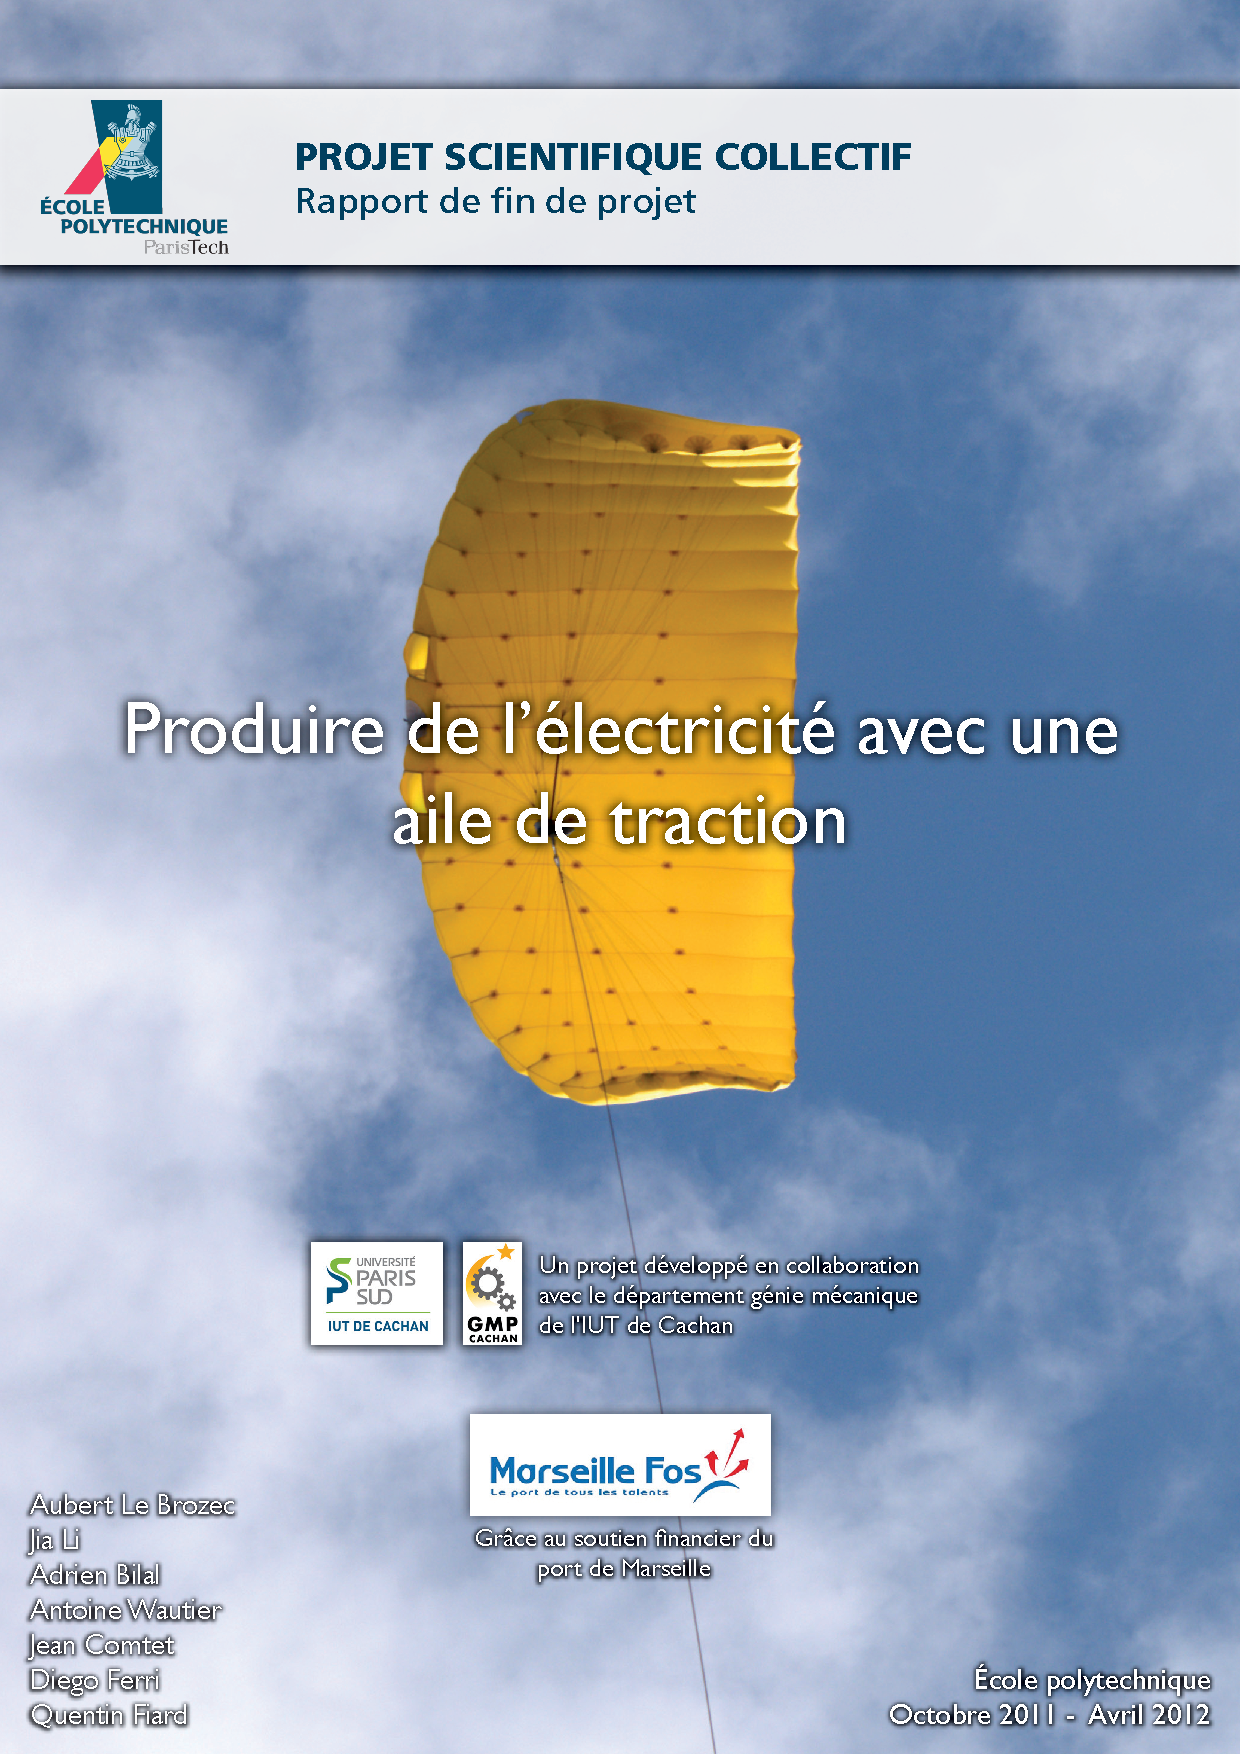
\includepdf{./images/page_de_garde.pdf}

\setlength{\hoffset}{\myhoffset}
\setlength{\voffset}{\myvoffset}

\newpage

\tableofcontents

\newpage

\begin{intro}
- poser le problème
- le problème en grandeur nature
- ce qui a déja été fait sur le sujet
- qques chiffres sur les cargos...
- approche énergétique
- insister sur le fait que c'est en plein boom
\end{intro}

\newpage

\begin{remerciements}

\end{remerciements}

\newpage



\begin{partie}{Physique de l'aile}

Modélisation du pb , notations, hypothèses (voile rigide, fils tendus et droits, bord d’attaque perp à la trajectoire)

\begin{sous-partie}{Modèle 2D}

\end{sous-partie}

\begin{sous-partie}{Étude qualitative de la dynamique (2D puis en se donnant une trajectoire)}

\end{sous-partie}

\begin{sous-partie}{Gerris, calcul des tables des coefficients aéro}

\end{sous-partie}

\end{partie}

\newpage

\begin{partie}{Description technique de l'expérience}

Nous avons défini notre problématique d'asservissement comme suit : Comment imposer au kite le suivi d'une trajectoire donnée ?
Plus précisément, notre objectif était de faire décrire une trajectoire en forme de huit à une aile de traction en notre possession (environ $2m^2$). %NL%
{lien avec les problèmes initiaux}
On entend ici par trajectoire la position absolue du kite dans l'espace, ainsi que son orientation spatiale. %NL%
Il y a donc théoriquement six variables indépendantes à mesurer : trois pour la position et trois pour l'orientation.\\
Toutefois, nous avons fait l'hypothèse que l'ensemble des positions atteintes par l'aile de kite, du fait de son attache au sol, est en 1ere approximation une sphère (du fait de la valeur faible de $\frac{l}{L} << 1$. %NL%
La position va de ce fait pouvoir être repérée par deux variables indépendantes uniquement (correspondant par exemple aux angles $\theta$ et $\phi$ en coordonnée sphériques, r étant fixé). %NL%
L'orientation spatiale va quant à elle pouvoir être décrite par une seule variable, que nous appellerons $\alpha$.


\begin{sous-partie}{Comment passer du problème réel au problème réduit ?}
- cargo + centrale : notre exp s'applique aux 2\\
- le boitier dont on étudie la conception sera en fait en l'air - analyse de la similitude des écoulements\\
- dimensionnement
\end{sous-partie}

\begin{sous-partie}{Cahier des charges}
- quelles grandeurs doit on mesurer ? %NL%
quelle précision ? %NL%
\\
- quelle vitesse de moteur ? %NL%
quelle précision ? %NL%
quel couple ? %NL%
\\
- quelle force va s'appliquer sur le système ? %NL%
quelle robustesse prévoir ? %NL%
\\
\\
- faire un tableau stylé avec les différentes précisions attendues.
\\
a)	Les actionneurs\\

Afin de piloter l'aile de traction, nous avions besoin d'un système capable de reproduire un pilotage humain, c'est à  dire un système d'actionneurs permettant de faire varier les longueurs relatives des deux lignes de l'aile de traction. %NL%
\\
Afin de faire varier les longueurs relatives des lignes, nous avons choisi d'utiliser un moteur unique entraînant un arbre sur lequel sont fixées une bobine permettant un enroulement des lignes en sens contraire (Cf. %NL%
figure 1). %NL%
Ainsi, lorsque l'on enroule une ligne, l'autre se déroule. %NL%
Ce système a deux avantages par rapport à une solution à deux moteurs :  \\
-	il permet de mettre en jeu des couples bien moindres car les couples exercés par les deux lignes sur l'axe qui se compensent approximativement en permanence (le couple résultant est négligeable par rapport au couple exercé par l'une des deux lignes). %NL%
\\
-	En déroulant une ligne pendant que l'on enroule l'autre, on fait varier plus rapidement les longueurs relatives des lignes que si l'on jouait sur une seule ligne à la fois, ce qui diminue le temps de réponse du système. %NL%
\\
\\
% Celui-ci doit pouvoir être commandé de deux façons différentes : d'une part de façon manuelle lors des phases de décollage et d'atterrissage de l'aile (au moyen d'un Joystick), et d'autre part de façon asservie (via le logiciel de simulation de l'écoulement) lors du suivi de trajectoire.\\
\\
 c) 	Choix de l'aile de traction \\
Les caractéristiques attendues de notre aile de traction devaient être les suivantes : \\
-	L'aile doit avoir deux lignes de traction de préférence (et non quatre), pour des raisons de complexité de l'asservissement et de simplicité de la commande.\\
-	L'aile doit être relativement rigide, étant donné que le logiciel de simulation de l'écoulement que nous utilisons calcul les coefficients pour un profil de voile rigide. %NL%
Ceci est assuré dès que le vent est suffisamment fort et régulier pour maintenir gonflés les caissons de l'aile et que le pilotage se fait sans à-coups et ??? %NL%
sans variation de la longueur des lignes de l'ordre de la taille de l'aile.??? %NL%
 \\
-	L'aile ne doit pas être trop grande ou trop puissante, pour être contrôlable via les actionneurs.\\
\\
e)	Mesure du vent\\
La mesure du vent relatif a été faite de façon indirecte en mesurant le vent au sol et en lui ajoutant la vitesse de l'aile en vol connue par dérivation de sa position par rapport au temps... %NL%

Un anémomètre et une girouette ont donc été intégrés aux boitier au sol.
\\
f)	Détermination de la position de l'aile de traction et capteur\\
L'asservissement reposant sur la trajectoire du kite, nous avons besoin de connaître plusieurs paramètres de vol de l'aile de traction : 
-	Le modèle aérodynamique développé par ailleurs nécessite la connaissance du vent relatif au niveau de l'aile pour calculer la trainée et la portance qui s'appliquent sur celle-ci.
-	Le suivi d'une trajectoire prédéfinie nécessite la connaissance de la position de l'aile de traction dans l'espace. %NL%
Celle-ci évoluant sur une sphère, la position de son centre de gravité est donnée par la mesure de deux angles, et la rotation propre de l'aile autour de l'axe moyen des deux lignes nécessite la connaissance d'un angle supplémentaire.
Comme évoquée dans le cahier des charges, la position de l'aile est déterminée par la connaissance de 3 angles  (deux angles pour son centre de gravité et un angle pour l'orientation de l'aile par rapport au fil qui la relie au sol).
On peut en déterminer deux en mesurant les angles de lacet et de tangage de la ligne qui relie l'aile de traction et la nacelle de l'actionneur à la terre. %NL%
Pour la mesure de ceux-ci, on décompose la liaison rotule entre la ligne partant de la nacelle et la terre en deux liaisons pivot superposées l'une à l'autre et munies chacune d'un capteur angulaire.

\end{sous-partie}


\begin{sous-partie}{Solutions apportées}

- partie électronique : circuits intégrés, capteurs, contrôle du moteur \\

- partie mécanique : moteur, anémomètre, prototypage rapide IUT Cachan, échec de l'AX- 18, travail du bois, caméra... %NL%
\\
\\

a) Principe général du boitier de contrôle



b) Production des pièces et réalisation du boitier\\
La réalisation du boitier de contrôle nécessitait de produire plusieurs pièces et de les assembler avec une précision plus ou moins grande. %NL%
Suite à notre collaboration avec Monsieur Martinelli, professeur à l'IUT de Cachan, nous avons décidé d'utiliser deux moyens de production pour réaliser nos pièces, à savoir : Une machine de prototypage rapide et une machine de découpe laser. %NL%
Le choix de ces moyens de production nous ont amenés à réaliser une modélisation sous solidedge de l'ensemble de notre système. %NL%
\\
La machine de prototypage rapide utilisé est … . %NL%
Elle fonctionne sur le principe… . %NL%
La production de pièces par cette machine est assez couteuse (1€/gramme de matière), nous l'avons donc utiliser pour réaliser les pièces demandant une grande précision, ou ayant une forme trop complexe pour être réalisée autrement.\\
La machine de découpe laser était une nouvelle acquisition de l'IUT, ce qui nous a permis d'inaugurer son utilisation pour une telle réalisation. %NL%
Un faisceau laser de puissance ??? %NL%
focalisé par une lentille, permet de découper des matériaux de différent type. %NL%
Nous avons de notre coté fait le choix du bois, de part son faible coût, et la facilité de sa découpe. %NL%
Cette machine combine donc les avantages d'une découpe très précise et d'un coût relativement faible de la production.\\
\\

d) Choix de l'actionneur\\
Nous nous sommes orientés dans un premier temps vers l'utilisation d'un servomoteur dynamixel AX-18, (puissance) contrôlable facilement de manière numérique. %NL%
En effet, ce servomoteur comporte des capteurs et une puce intégré, qui permettent de l'asservir très facilement en position, et d'obtenir en retour certaines informations sur son état de fonctionnement (vitesse de rotation, couple exercé sur l'axe moteur, température du moteur...) Cf. %NL%
Annexe : doc technique de l'AX-18. %NL%
Les interactions avec le moteur se font via l'envoi de paquet... %NL%
Nous avons donc dans un premier temps choisi de travailler avec un tel actionneur, et réalisé un premier prototype. %NL%
Cependant, suite à une manipulation peu heureuse, le moteur s'est cassé.\\
Nous nous sommes donc tourné vers le choix d'un second actionneur, plus robuste et moins cher. %NL%
Nous avons ainsi acquis un Hyperion ZS 2213 22, couplé avec un réducteur planétaire Maxon 53 :1. %NL%
(indiquer la puissance). %NL%
Malgré ses très bonnes caractéristiques, ce moteur est assez difficilement contrôlable en position, car ... %NL%
. %NL%
Nous nous sommes donc tournés vers un asservissement en P.I.D. %NL%
en vitesse du moteur, ce qui permet tout de même un contôle manuel de la voile via joystick. %NL%
D'autre part, étant donné la structure de l'asservissement sous Acado mis en place, un asservissement en vitesse était plus intéressant.
\\

e) Choix des capteurs\\
La mesure des angles sera obtenue via des capteurs magnétiques AS5045.\\
Un système de guide-fil redirige les câbles et permet de mesurer l'inclinaison des fils et donc d'obtenir une mesure des angles $\theta$ et $\phi.$. %NL%
La majorité du système est réalisé en bois...
Après validation de notre solution par Monsieur Martinelli, nous souhaitons si c'est possible réaliser les pièces du guide-fil au département de génie mécanique de l'IUT de Cachan. %NL%
Du fait de la grande précision nécessaire concernant la position aimant/capteur angulaire, nous souhaitons réaliser une partie de ces pièces par prototypage rapide. %NL%
Etant depuis peu sponsorisé par le port de Marseille, nous pouvons apporter à l'IUT un dédommagement financier concernant le matériel prêté.\\
Pour déterminer l'angle de rotation de l'aile de traction autour de la ligne principale, la solution envisagée passe par du traitement d'images. %NL%
Une caméra au sol tournant avec l'aile et pointant ainsi toujours dans l'axe de la ligne reconnaîtra un motif caractéristique sur l'aile (une bande fluo par exemple) et mesurera l'angle de rotation de celui-ci autour de l'axe de la ligne (cette caméra est représentée sur la figure 7). %NL%
Nous comptons utiliser une caméra en notre possession pour réaliser cette mesure. %NL%
Ceci impliquera un traitement de l'image en temps réel. %NL%
Le principal problème technique auquel nous sommes confrontés est de synchroniser la caméra avec le fil qui relie la nacelle au sol (il faut que la caméra suive la nacelle dans son vol). %NL%
Nous comptons utiliser une webcam haute résolution, qui est déjà en notre possession (Logitech Cam C210).

\end{sous-partie}

\begin{sous-partie}{Démarches}
- IUT Cachan\\
- Sponsor Port de Marseille, création d"un binet, plaquette sponsors - concours energia\\
\end{sous-partie}




\end{partie}

\newpage

\begin{partie}{Contrôle numérique du système}
Intro (ou dans III.2) : schéma d'asservissement pour rappeler quelles grandeurs on commande, quelles grandeurs on mesure + schéma couche par  couche comme dans la thèse

\begin{sous-partie}{Système informatique de suivi de l'expérience}

\begin{sous-sous-partie}{Conception de l'architecture du système informatique}

\begin{paragraph}{Cahier des charges\vspace{0.3cm}\\}
La composante logicielle du projet doit être à même d'exécuter l'algorithme de contrôle optimal qui permet d'asservir l'aile sur une trajectoire donnée. %NL%
Pour remplir cette mission, elle doit satisfaire aux besoins suivants :
\begin{liste}
\item Gérer une interface entre l'algorithme et les différents capteurs qui nous renseignent sur l'état de l'aile en temps réel.
\item Transmettre au moteur la commande calculée par l'algorithme.
\item Offrir une interface utilisateur permettant le suivi en temps réel de l'expérience.
\item Enregistrer les données recueillies pendant un essai, pour permettre leur exploitation.
\end{liste}
\end{paragraph}

\begin{paragraph}{Architecture informatique choisie\vspace{0.3cm}\\}
Pour répondre à ces besoins, nous avons décidé de séparer le système informatique en deux composantes distinctes. %NL%

\begin{liste}
\item Un module, embarquée sur une carte électronique, gère l'acquisition en temps réel des données des capteurs angulaires, le contrôle et l'asservissement en vitesse du moteur.
\item Un second module, exécuté sur un ordinateur portable, prend en charge l'interface utilisateur, le traitement des images en provenance de la caméra, l'enregistrement des données, et l'exécution de l'algorithme d'asservissement, point névralgique du projet.
\end{liste}
La figure~\ref{archinfo} illustre cette répartition des tâches.
\end{paragraph}

\begin{figure}[htb]
	\centering
	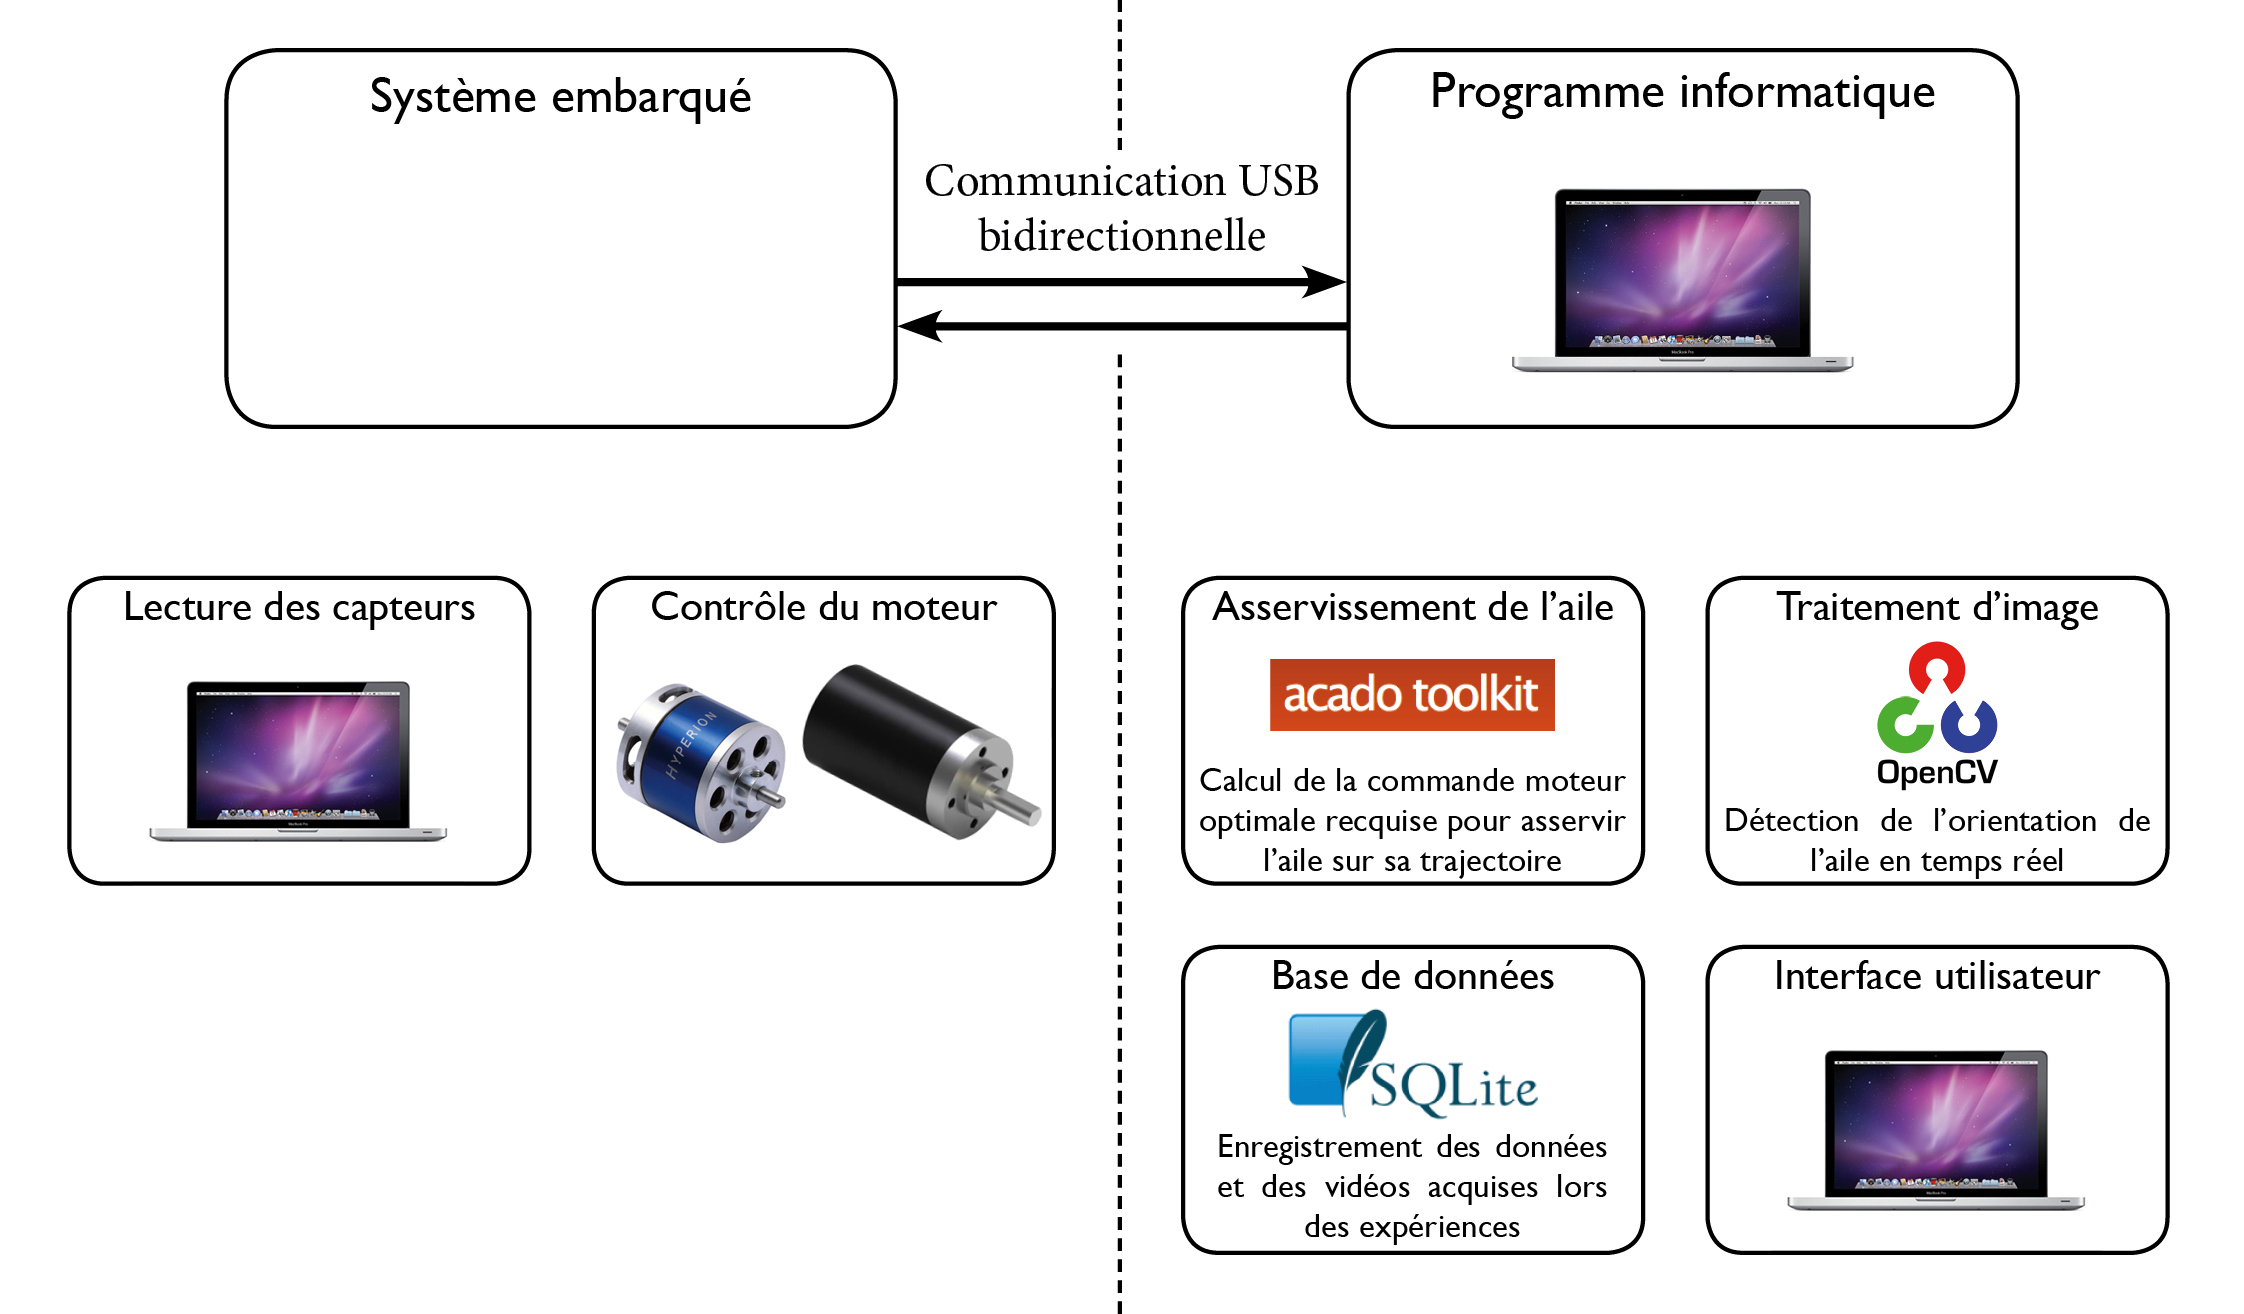
\includegraphics[width=\linewidth]{./images/architecture_logicielle.jpg}
	\caption{Architecture globale de la composante informatique du projet}
	\label{archinfo}
\end{figure}

\end{sous-sous-partie}

\begin{sous-sous-partie}{Conception de la composante embarquée du système informatique}

\begin{paragraph}{Cahier des charges\vspace{0.3cm}\\}
Comme présentée dans la section précédente, nous avons donc été confronté lors de la conception du prototype au besoin d'une interface entre d'une part les capteurs angulaires et le moteur, qui nous permettent d'avoir un retour direct sur le bon déroulement de l'expérience et une action correctrice sur l'aile en vol, et d'autre part l'ordinateur qui exécute l'algorithme d'asservissement, et qui requiert des informations en temps réel sur l'état du système. %NL%
Le cahier des charges que nous avons établi pour cette composante est donc le suivant :
\begin{liste}
\item Acquérir en temps réel les données en provenance de cinq capteurs angulaires à effet Hall de type AS5045, produit par austriamicrosystems.
\item Contrôler et asservir en vitesse un moteur par le biais d'un protocole en modulation d'impulsion codée (décrit dans la suite du rapport, et utilisé très largement en modélisme).
\item Pouvoir se connecter aisément et échanger à haut débit des données avec un ordinateur.
\end{liste}
\end{paragraph}

\begin{paragraph}{\mbox{Solution technique retenue\vspace{0.3cm}\\}}
\begin{subparagraph}{}
Afin d'avoir une liberté et un contrôle maximaux sur les données échangées et leur traitement, et devant l'absence de composants sur étagère adaptés, nous avons décidé de développer notre propre carte électronique permettant de remplir les exigences opérationnels listées.
\end{subparagraph}

\begin{subparagraph}{}
La carte que nous avons conçue est capable d'acquérir des données provenant de jusqu'à six capteurs angulaires, et contrôler jusqu'à quatre moteurs, et d'en asservir un en vitesse. %NL%
La carte peut se connecter en USB à un ordinateur, avec un débit d'environ 125 kbits/s. %NL%
Elle s'articule autour d'un microcontrôleur PIC18F2550, de marque Microchip, choisi pour sa gestion de l'interface USB, son nombre de ports suffisants pour les besoins de l'application, et sa puissance de calcul relativement conséquente (12 millions d'opérations élémentaires par seconde).
\end{subparagraph}
\end{paragraph}

\begin{paragraph}{Conception du circuit électronique\vspace{0.3cm}\\}
Nous avons dessiné le schéma du circuit électronique de la carte sur Eagle, un logiciel de conception de circuit imprimé développé par la société CadSoft, dont une version limitée est disponible gratuitement en ligne. %NL%
La figure~\ref{schemaCircuitCarte} présente la version finale du circuit qui a été ensuite gravée pour réaliser la carte électronique. %NL%
Outre les composants nécessaires au fonctionnement du microcontrôleur (condensateurs de découplage, quartz d'horloge), nous avons ajouté un port USB pour la connection à l'ordinateur, et un certain nombre de prises pour les connections aux capteurs et aux moteurs.
\end{paragraph}

\begin{figure}[hbt]
	\centering
	\includegraphics[width=\linewidth]{./images/schema_circuit_carte.eps}
	\caption{Schéma du circuit électronique de la carte d'acquisition}
	\label{schemaCircuitCarte}
\end{figure}

\FloatBarrier

\begin{paragraph}{Fabrication du circuit imprimé\vspace{0.3cm}\\}

La fabrication du circuit à partir du schéma électronique s'est alors effectuée en plusieurs étapes.
\begin{liste}
\item À l'aide du logiciel Eagle, nous avons pu transformer le schéma que nous avions défini en un circuit imprimé double couche, supportant le microcontrôleur dans sa version CMS (composant monté en surface), ainsi que les autres composants.
\item À partir du circuit ainsi créé, nous avons imprimé un typon à l'échelle 1 sur une imprimante jet d'encre, à même d'être gravé sur une plaque cuivrée présensibilisée.
\begin{figure}[!h]
	\centering
	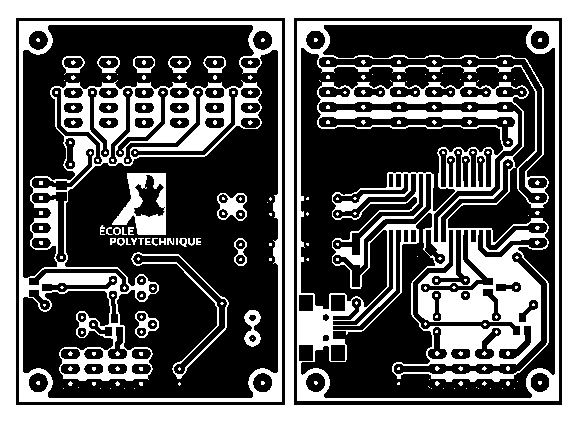
\includegraphics[scale=1]{./images/circuit_imprime_carte.eps}
	\caption{Typon à l'échelle 1 dessiné sous Eagle du circuit imprimé de la carte d'acquisition}
	\label{circuit_imprime_carte}
\end{figure}
\item A l'aide d'une insoleuse à tube UV, le circuit est flashé sur la plaque de cuivre, qui est ensuite développée dans une solution peu concentrée de soude. Dans les régions transparentes du typon, le vernis protecteur est alors dissous, et le cuivre est directement visible.
\item L'excédent de cuivre (où le vernis protecteur a été dissous) est alors oxydé dans une solution composée de 10\% de peroxyde d'oxygène (eau oxygénée à 130 volumes), 10\% d'acide chlorhydrique à 23\%, et 80\% d'eau, en prenant garde à la sécurité des manipulations (port de gants et d'une blouse).

\end{liste}
\end{paragraph}

\begin{paragraph}{Programmation du microcontrôleur\vspace{0.3cm}\\}
Le programme du microcontrôleur a été écrit en C sous l'environnement de développement MPLAB~X, développé par Microchip. %NL%
Nous allons maintenant présenter comment nous sommes parvenus à réaliser l'acquisition des données des capteurs et la commande du moteur.

\begin{subparagraph}{Acquisition des données des capteurs.}
La fiche technique du capteur AS5045 présente le protocole de communication permettant de lire la position angulaire mesurée par le capteur (figure~\ref{protocole_capteur}). %NL%
Il s'agit d'un protocole de communication en série, où le capteur envoie un bit de donnée à chaque fois qu'il reçoit un signal horloge du microcontrôleur. %NL%
Un paquet de données est formée de 12 bits qui représentent la position angulaire (soit 4096 positions par tours), suivis de 6 bits donnant le status du capteur et permettant de détecter des erreurs de communication. %NL%
Un port du capteur est de plus utilisé pour choisir de quel capteur nous souhaitons lire les données, ce qui permet de lire les six capteurs avec seulement 8 ports sur le microcontrôleur (6 ports de sélection, un d'horloge, et un de lecture).

\begin{figure}[!h]
	\centering
	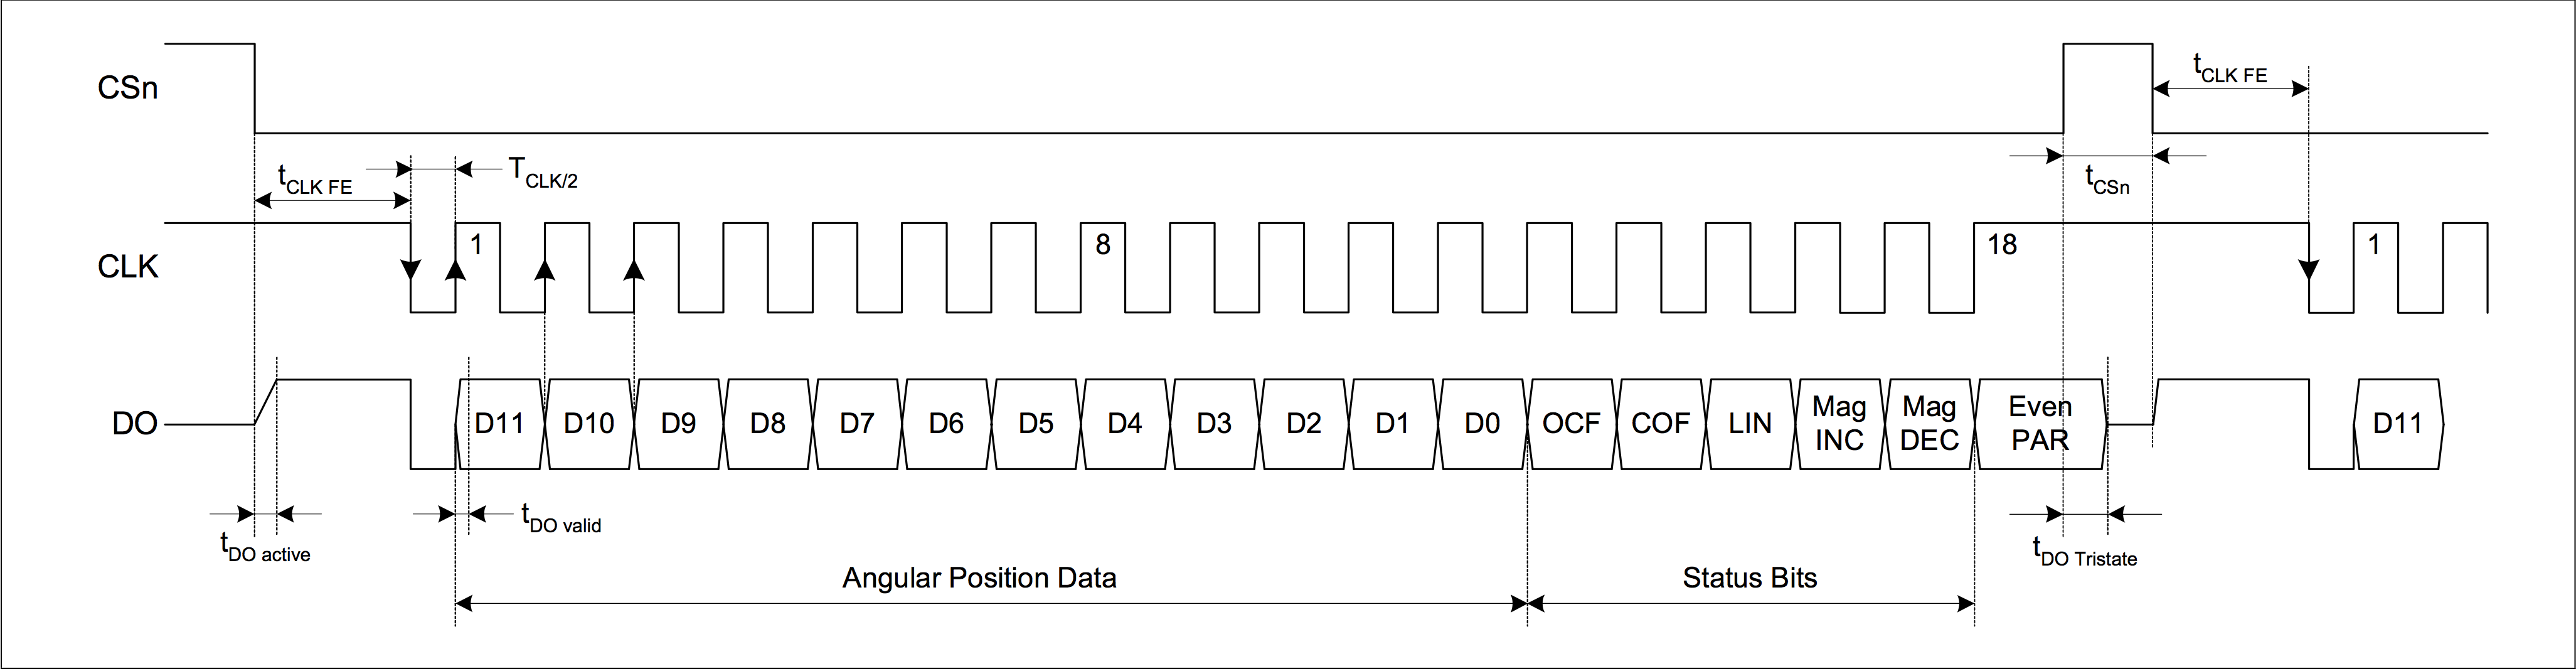
\includegraphics[width=\textwidth]{./images/protocole_capteur.png}
	\caption{Protocole de communication utilisés par les capteurs angulaires}
	\label{protocole_capteur}
\end{figure}

Ce protocole a été implémenté dans le microcontrôleur, et la figure~\ref{protocole_capteur_oscillo} présente la réponse réelle d'un capteur suite à une interrogation du microcontrôleur, telle que vue sur un oscilloscope.

\begin{figure}[!h]
	\centering
	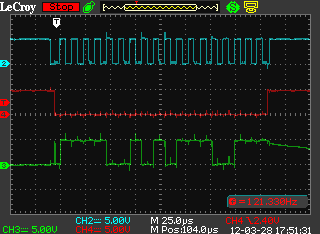
\includegraphics[width=10cm]{./images/protocole_capteur_oscillo.png}
	\caption{\textbf{\color{Cerulean}Signal d'horloge}, de \textbf{\color{Red}sélection de capteur} et de \textbf{\color{ForestGreen}réponse du capteur} lors d'une acquisition de données angulaires.}
	\label{protocole_capteur_oscillo}
\end{figure}

\end{subparagraph}

\begin{subparagraph}{Contrôle et asservissement du moteur}
Le moteur est contrôlé par un signal en modulation d'impulsion codée. %NL%
Largement répandu en modélisme, ce signal se caractérise par l'encodage de la commande sous forme d'une pulsation dont la largeur est corrélée à la commande, émis à une fréquence qui ne dépend pas de la commande, et qui de l'ordre de 50 Hz. %NL%
Du fait de sa vitesse d'exécution de 12 millions d'opérations par seconde et de sa grande précision temporelle, le microcontrôleur choisi est tout à fait adapté pour générer de tels signaux. %NL%
Les figures~\ref{signal_pcm_global}~et~\ref{signal_pwm_detail} illustrent la forme des signaux générés par le microcontrôleur pour le contrôle du moteur. %NL%


\newlength{\largeurphotooscillo}
\setlength{\largeurphotooscillo}{\textwidth}
\addtolength{\largeurphotooscillo}{-0,6cm}
\setlength{\largeurphotooscillo}{\largeurphotooscillo/2}

\begin{figure}[!h]
	\centering
	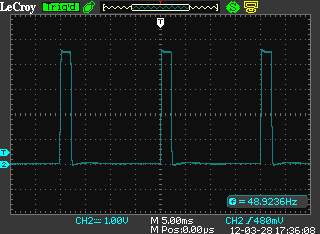
\includegraphics[width=\largeurphotooscillo]{./images/signal_pcm_global.png}
	\caption{La fréquence d'émission des pulsations est de l'ordre de 50 Hz}
	\label{signal_pcm_global}
\end{figure}

\begin{figure}[!h]
	\centering
	\captionsetup[subfigure]{labelformat=empty}
	\subfloat[Moteur à l'arrêt]{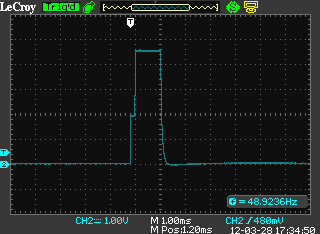
\includegraphics[width=\largeurphotooscillo]{./images/signal_pcm_neutre.png}}
	\hspace{0,5cm}\subfloat[Moteur en rotation à la vitesse maximale dans le sens positif]{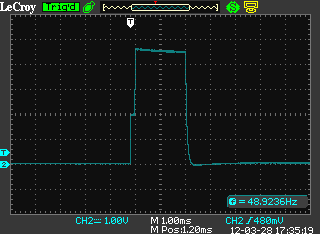
\includegraphics[width=\largeurphotooscillo]{./images/signal_pcm_max.png}}
	\caption{Variation de la largeur d'impulsion en fonction de la commande}
	\label{signal_pwm_detail}
\end{figure}

\end{subparagraph}

\end{paragraph}

\end{sous-sous-partie}

\end{sous-partie}



\begin{sous-partie}{Calcul des coéfficients aérodynamiques via Gerris}

\end{sous-partie}

\begin{sous-partie}{Description théorique de l'asservissement}
La trajectoire en 8 que nous souhaitons faire suivre à notre aile de traction-trajectoire que nous avons nous-mêmes déterminée à l'aide d'un algorithme d'optimisation comme on pourra le voir en partie IV- n'est pas une trajectoire auto-stable : sans contrôle, l'aile de Kite surf ne peut rester dessus. %NL%
Il y a donc besoin d'un contrôle en permanence au niveau de la longueur des câbles pour que l'aile puisse suivre cette trajectoire. %NL%

\newline
Par ailleurs, on ne peut enregistrer une séquence d'asservissement en avance pour l'imposer ensuite à l'aile. %NL%
En effet, les vents étant relativement changeants, les commandes que l'on donne à l'aile doivent être adaptées au conditions climatiques à tout instant.
\newline
C'est pourquoi un asservissement en temps réel de la position de l'aile est indispensable.
Rappelons que nous considérons dans cette étude que l'aile vole sur une sphère de rayon r fixé ($r=20m$ pour notre expérience, $R=600 m$ pour les systèmes d'ailes de traction sur cargos) et que nous connaissons la position de l'aile grâce aux mesures des angles $\theta$ et $\phi$ (via des capteurs incrémentaux au niveau de la liaison de l'aile avec le sol) ainsi que son orientation décrite par les angles $\psi_1$ et $\psi_2$ (l'angle  $\psi_1$ est connu directement à partir du différentiel de longueur entre les 2 brins, et $\psi_2$ est obtenu à l'aide de traitement d'image par caméra).
Par ailleurs, nous disposons également des dérivées de ces 4 grandeurs en calculant des taux d'accroissement à intervalles de temps petits (suffisamment petits pour que l'incertitude due à ces calculs ne soit pas dominante, comme on l'explique dans la suite). %NL%
En pratique, comme nous allons le voir dans la suite, nous n'avons pas besoin de connaître les grandeurs $\dot{\psi_1}(t)$ et $\dot{\psi_2}(t)$ pour l'asservissement.
\newline
La fonction d'état du Kite s'écrit alors :
$$X(t)=(\theta(t),\phi(t),\dot{\theta}(t),\dot{\phi}(t),\psi_1(t), \psi_2(t))^T$$
Il faut à présent définir le contrôle $u$ que l'on a sur le système. %NL%
Expérimentalement, nous avons pu constater le fait qu'il est possible de faire faire des 8 bouclés au Kite en agissant uniquement sur le différentiel de longueur entre les 2 brins. %NL%
Nous prenons donc pour grandeur de contrôle u la grandeur $\dot{\psi_1}(t)$ qui est directement reliée au différentiel de vitesse entre les deux brins et donc à la vitesse de rotation du moteur.
\newline
\begin{huge}
Insérer schéma Aubert 1 
\end{huge}
(et introduire les grandeurs x et L)
\newline
Comme $L x \cos \psi_1(t) = l_1 l_2 -r^2 +\frac{L^2}{4}$ alors : $$\psi_1(t) \approx \arccos \big[\frac{1}{2} + \frac{2(l_1 l_2-r^2)}{L^2}\big]-\pi$$ donc
$$u = \dot{\psi_1}(t)= -\frac{2\frac{d}{dt}[l_1(t) l_2(t)]}{L^2}* \frac{1}{1/2}$$ car $$1-(\frac{1}{2} + \frac{2(l_1 l_2-r^2)}{L^2})^2 = 1-\frac{1}{4} - 2 \frac{l_1(t)l_2(t)}{L^2} + \big(4 \frac{l_1(t)l_2(t)}{L^2}\big)^2 \approx \frac{3}{4}-\frac{1}{2} + \frac{1}{4}= \frac{1}{2}$$
On calcule : $\frac{d}{dt}[l_1(t) l_2(t)] = (\dot{l_1}(t)+ \dot{l_2}(t))\frac{l_1 + l_2}{2}+(\dot{l_1}(t)- \dot{l_2}(t))\frac{l_2 - l_1}{2}$. %NL%
Comme $l_1(t)+l_2(t)=C^{te}$, on a alors $\frac{d}{dt}[l_1(t) l_2(t)]= (\dot{l_1}(t)- \dot{l_2}(t))\frac{l_2 - l_1}{2}$, d'où :
$$u =  \frac{2 (\dot{l_1}(t)-\dot{l_2}(t))(l_1(t)+l_2(t))}{L^2} \approx \frac{4 r \dot{\mathcal{M}} R_{arbre moteur}}{L^2}$$ où $\dot{\mathcal{M}}$ est la vitesse du moteur (en pratique, c'est ce que l'on contrôle directement dans l'expérience.



On définit ensuite une fonction distance qui permet de voir de combien l'aile de traction s'est éloignée de la trajectoire prévue initialement (éloignement suite à changement brutal de vent, incertitudes dans le repérage de la position, inexactitudes dans l'asservissement en temps réel...). %NL%
Notons f cette fonction. %NL%
Il est à noter que, si l'algorithme effectue le calcul de la commande tous les $\Delta t$ (et applique la commande précédente pendant qu'il calcule la nouvelle), l'algorithme doit minimiser f non pas en une itération, mais pendant sur  une période de temps bien choisie (appelée horizon, notée $T_H$), pour éviter les phénomènes d'oscillation décrits par la figure suivante : 
\newline
\begin{Huge}
insérer schéma 2 (oscillations)
\end{Huge}
\newline
Le principe de l'asservissement en temps direct est alors le suivant : au temps t, on calcule (à l'aide d'un algorithme d'optimisation) liste de commandes à effectuer $(u_1,u_2,...)$ qui va permettre de minimiser (sur la durée $T_H$) la distance entre la trajectoire effective du Kite, et la trajectoire à suivre. %NL%
Si on calcule N commandes différentes pour le temps $T_H$, ceci signifie que le moteur va changer d'allure tous les $\frac{T_H}{N}s$ pour garder le kite sur la trajectoire. %NL%
Pendant que le moteur applique ces commandes, on en calcule une nouvelle série de façon à ce que le moteur tourne en continu. %NL%
Cette procédure est résumée sur le schéma suivant : 
\newline
\begin{huge}
insérer schéma 3 (pas de temps)
\end{huge}
Remarque : la durée $\delta t$ doit être choisie petite pour la précision de l'algorithme, pas trop petite non plus pour que le temps de calcul reste raisonnable et pour que le moteur ait le temps de réagir à chacune de ces modifications de sa vitesse.
\end{sous-partie}

\begin{sous-partie}{Acado et asservissement en temps réel}
Sur les conseils de Pierre Martinon (Chercheur au CMAP), nous avons utilisé le code Acado Toolkit, développé par Moritz Diehl, pour réaliser notre asservissement en temps réel, qui est un code crée spécifiquement pour ce genre de problème (Moritz Diehl a d'ailleurs étudié personnellement la production d'énergie à l'aide d'ailes de traction).
Son collaborateur Mario Zanon a accepté de nous aider à distance en nous guidant sur le débugage de problèmes internes à Acado.

Nous allons à présent évoquer deux points : les pas de temps que nous nous sommes fixés en pratique et la précision des calculs que nous avons réalisé.


- problème de détermination de l'horizon de temps (pour être assez précis et pour que le temps de calcul ne soit pas trop long
\\
- déterminer le pas de temps de l'algo (compromis entre précision et capacités des composants physiques) + la précision à laquelle on doit faire les calculs
\end{sous-partie}


\end{partie}

\newpage

\begin{partie}{Analyse de l'expérience et élargissement}

\begin{sous-partie}{Contrôle de l'aile via joystick et via asservissement}

\end{sous-partie}

\begin{sous-partie}{Limites du modèle réduit }
Pourquoi l'expérience est difficile à réaliser
\\
- aile souple
\\
- déformation des fils
\\
- inertie du moteur
\\
- vent instable, non horizontal
\\
- imprécision de calcul des coefficients ?
\\
Pourquoi l'expérience ne cadre pas tout à fait avec le modèle réel
- similitude de l'écoulement ?
\\
- boitier qui n'est pas en l'air
\end{sous-partie}

\begin{sous-partie}{Approche énergétique}
On a vu qu'il est possible de réaliser  l'asservissement d'une aile de traction.
\\
Comment mettre ceci à profit pour avoir le plus d'énergie possible ?
\\
Trajectoires optimales, robustesse.
\end{sous-partie}

\end{partie}

\newpage

\begin{biblio}

\end{biblio}

\begin{annexes}

\begin{annexe}{Fabrication des circuits imprimés}

\begin{figure}[!h]
	\captionsetup[subfigure]{labelformat=empty}
	\centering
	\newlength{\largeurphoto}
	\newlength{\margesphoto}
	\setlength{\margesphoto}{1cm}
	\setlength{\largeurphoto}{\linewidth/2}
	\addtolength{\largeurphoto}{-\margesphoto/2-0,1cm}
	\subfloat[Typon du circuit imprimé]{\includegraphics[width=\largeurphoto]{./images/capteurs_typon.jpg}}
	\hspace{\margesphoto}
	\subfloat[Après révélation, le cuivre est apparent dans les zones où le typon était transparent.]{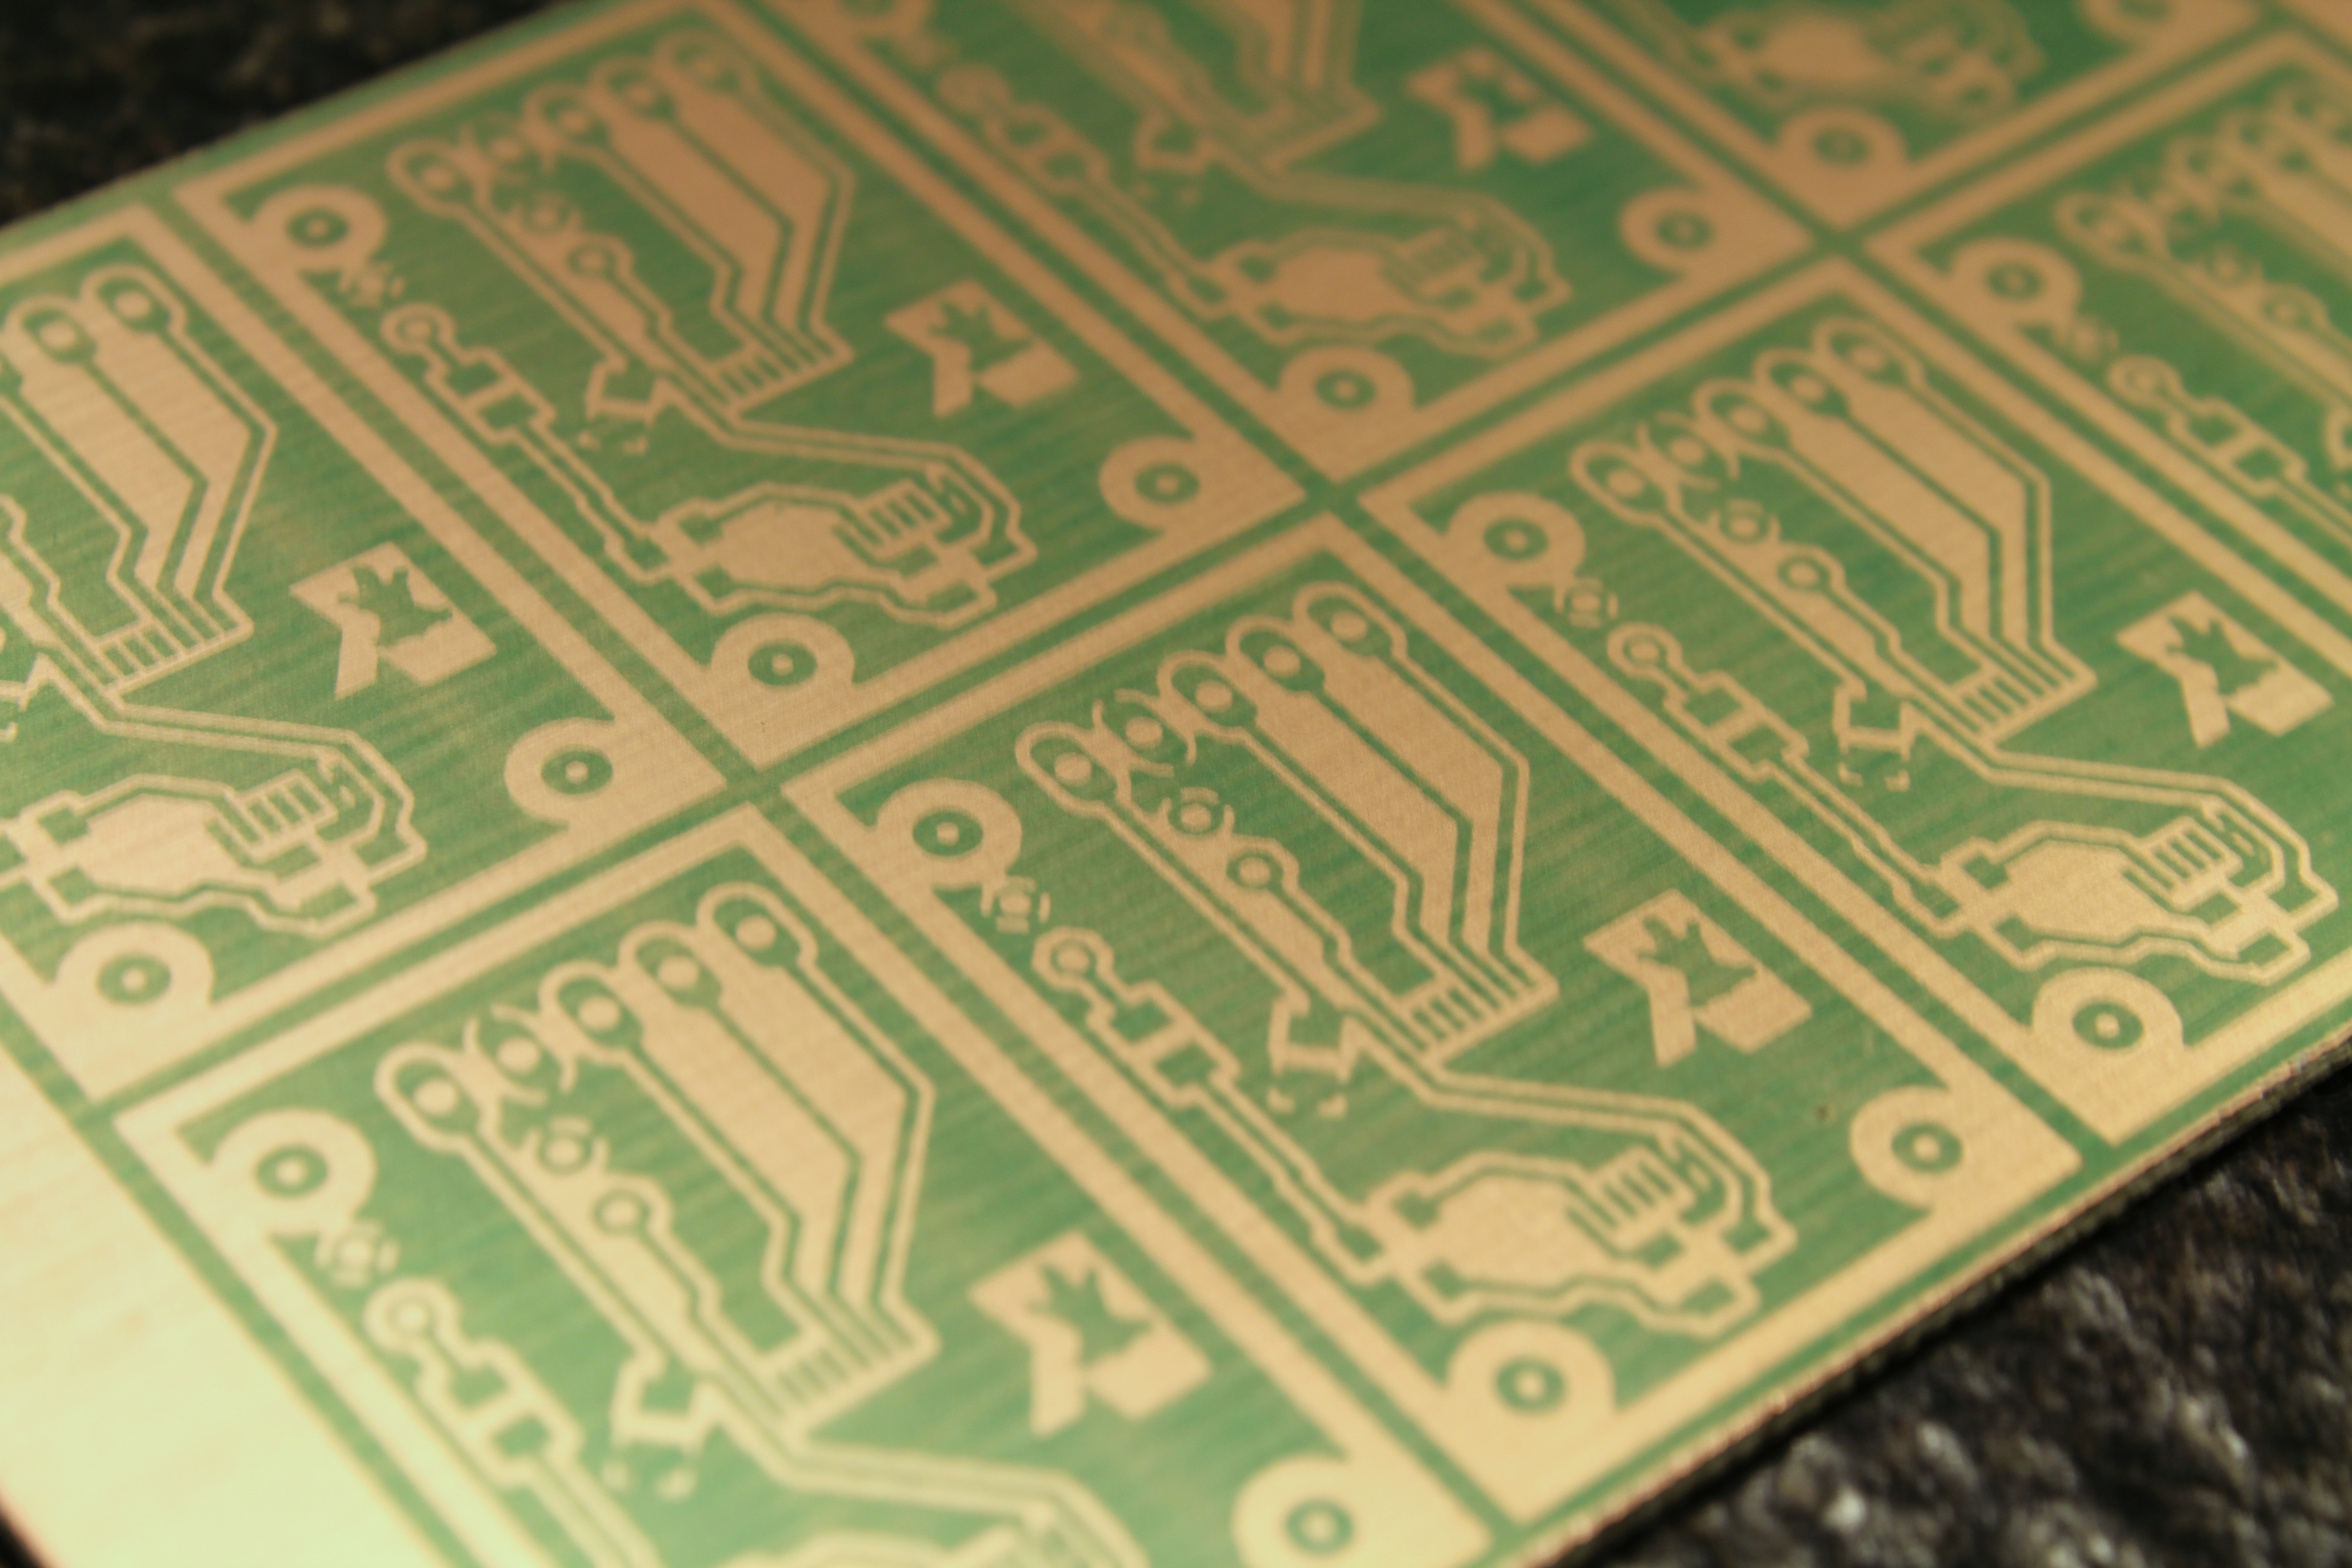
\includegraphics[width=\largeurphoto]{./images/capteurs_revelation.jpg}}\vspace{0.5cm}\\
	\subfloat[En cours de gravure. %NL%
Le cuivre non protégé est oxydé par la solution de peroxyde d'oxygène, dans une réaction exothermique.]{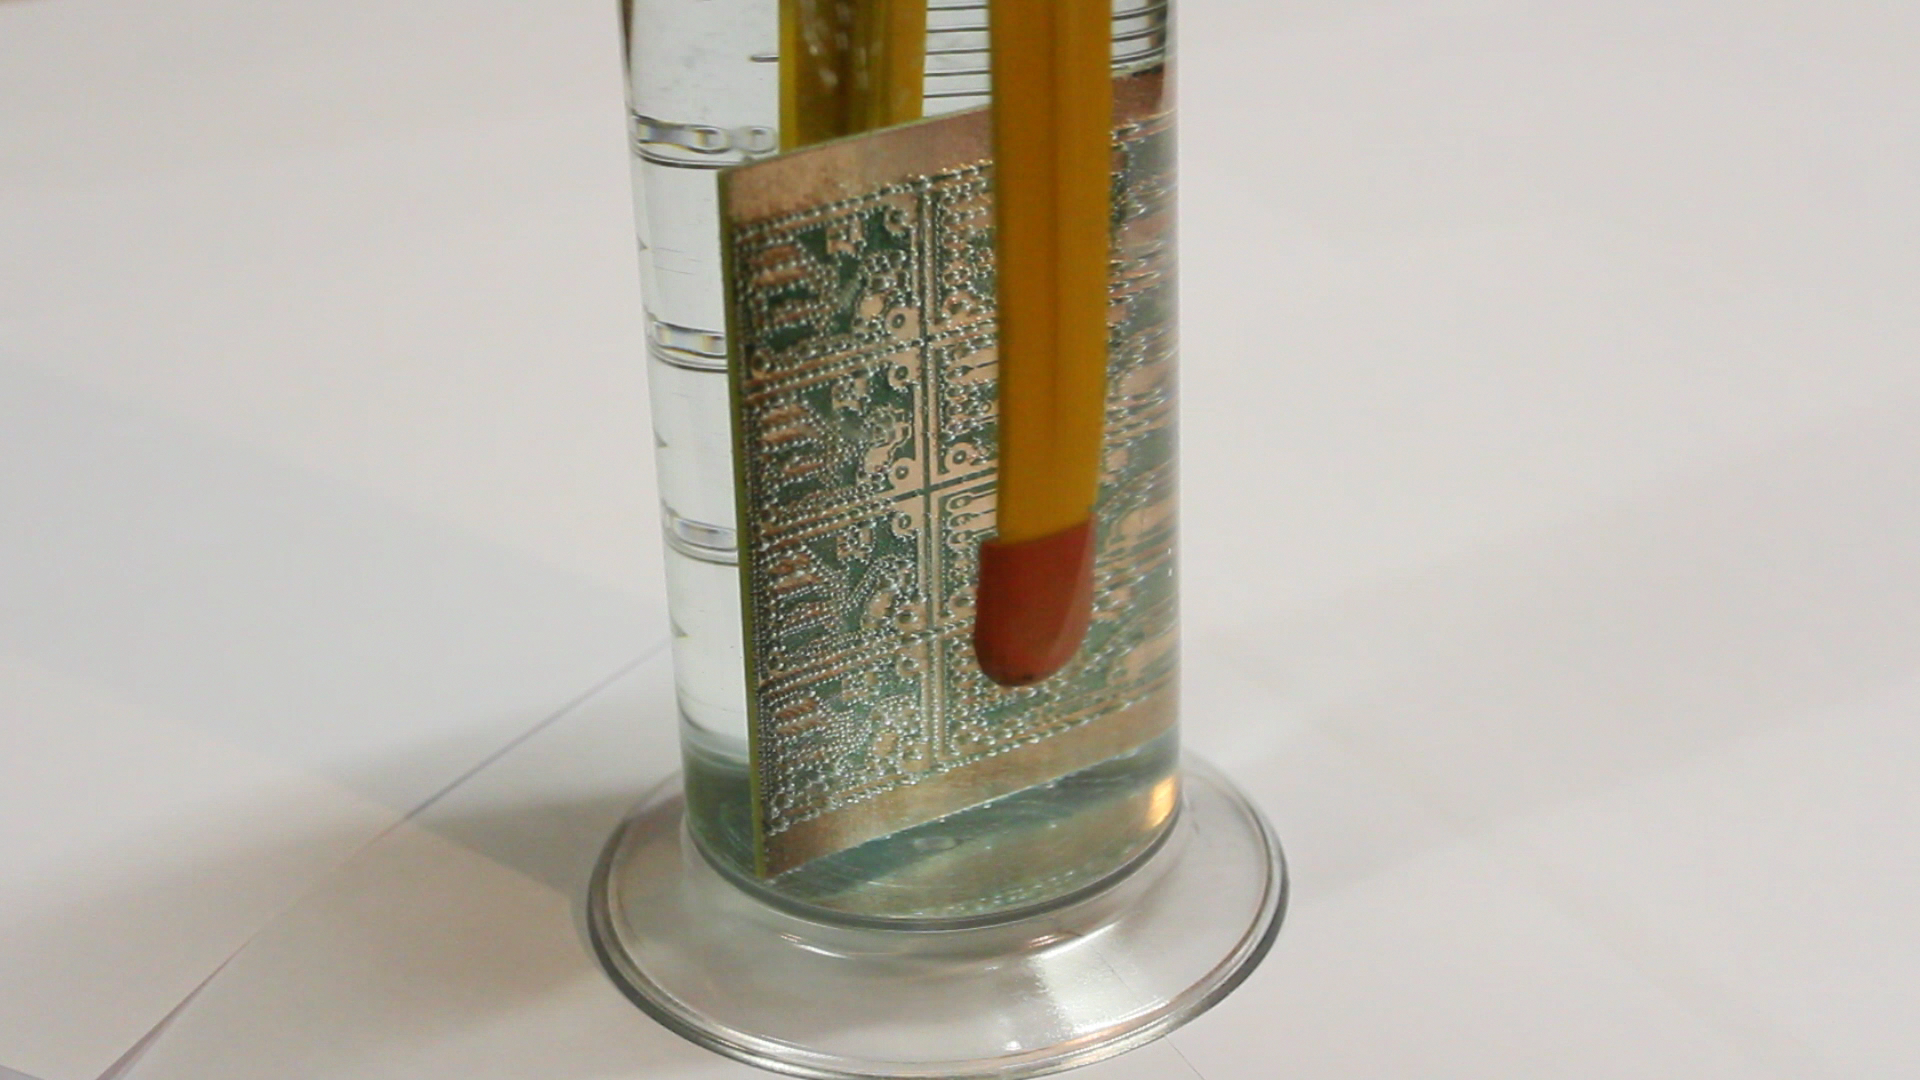
\includegraphics[width=\largeurphoto]{./images/capteurs_gravure.png}}
	\hspace{\margesphoto}
	\subfloat[Après gravure, le cuivre a été entièrement dissous, et n'est plus présent que dans les zones où le typon était opaque.]{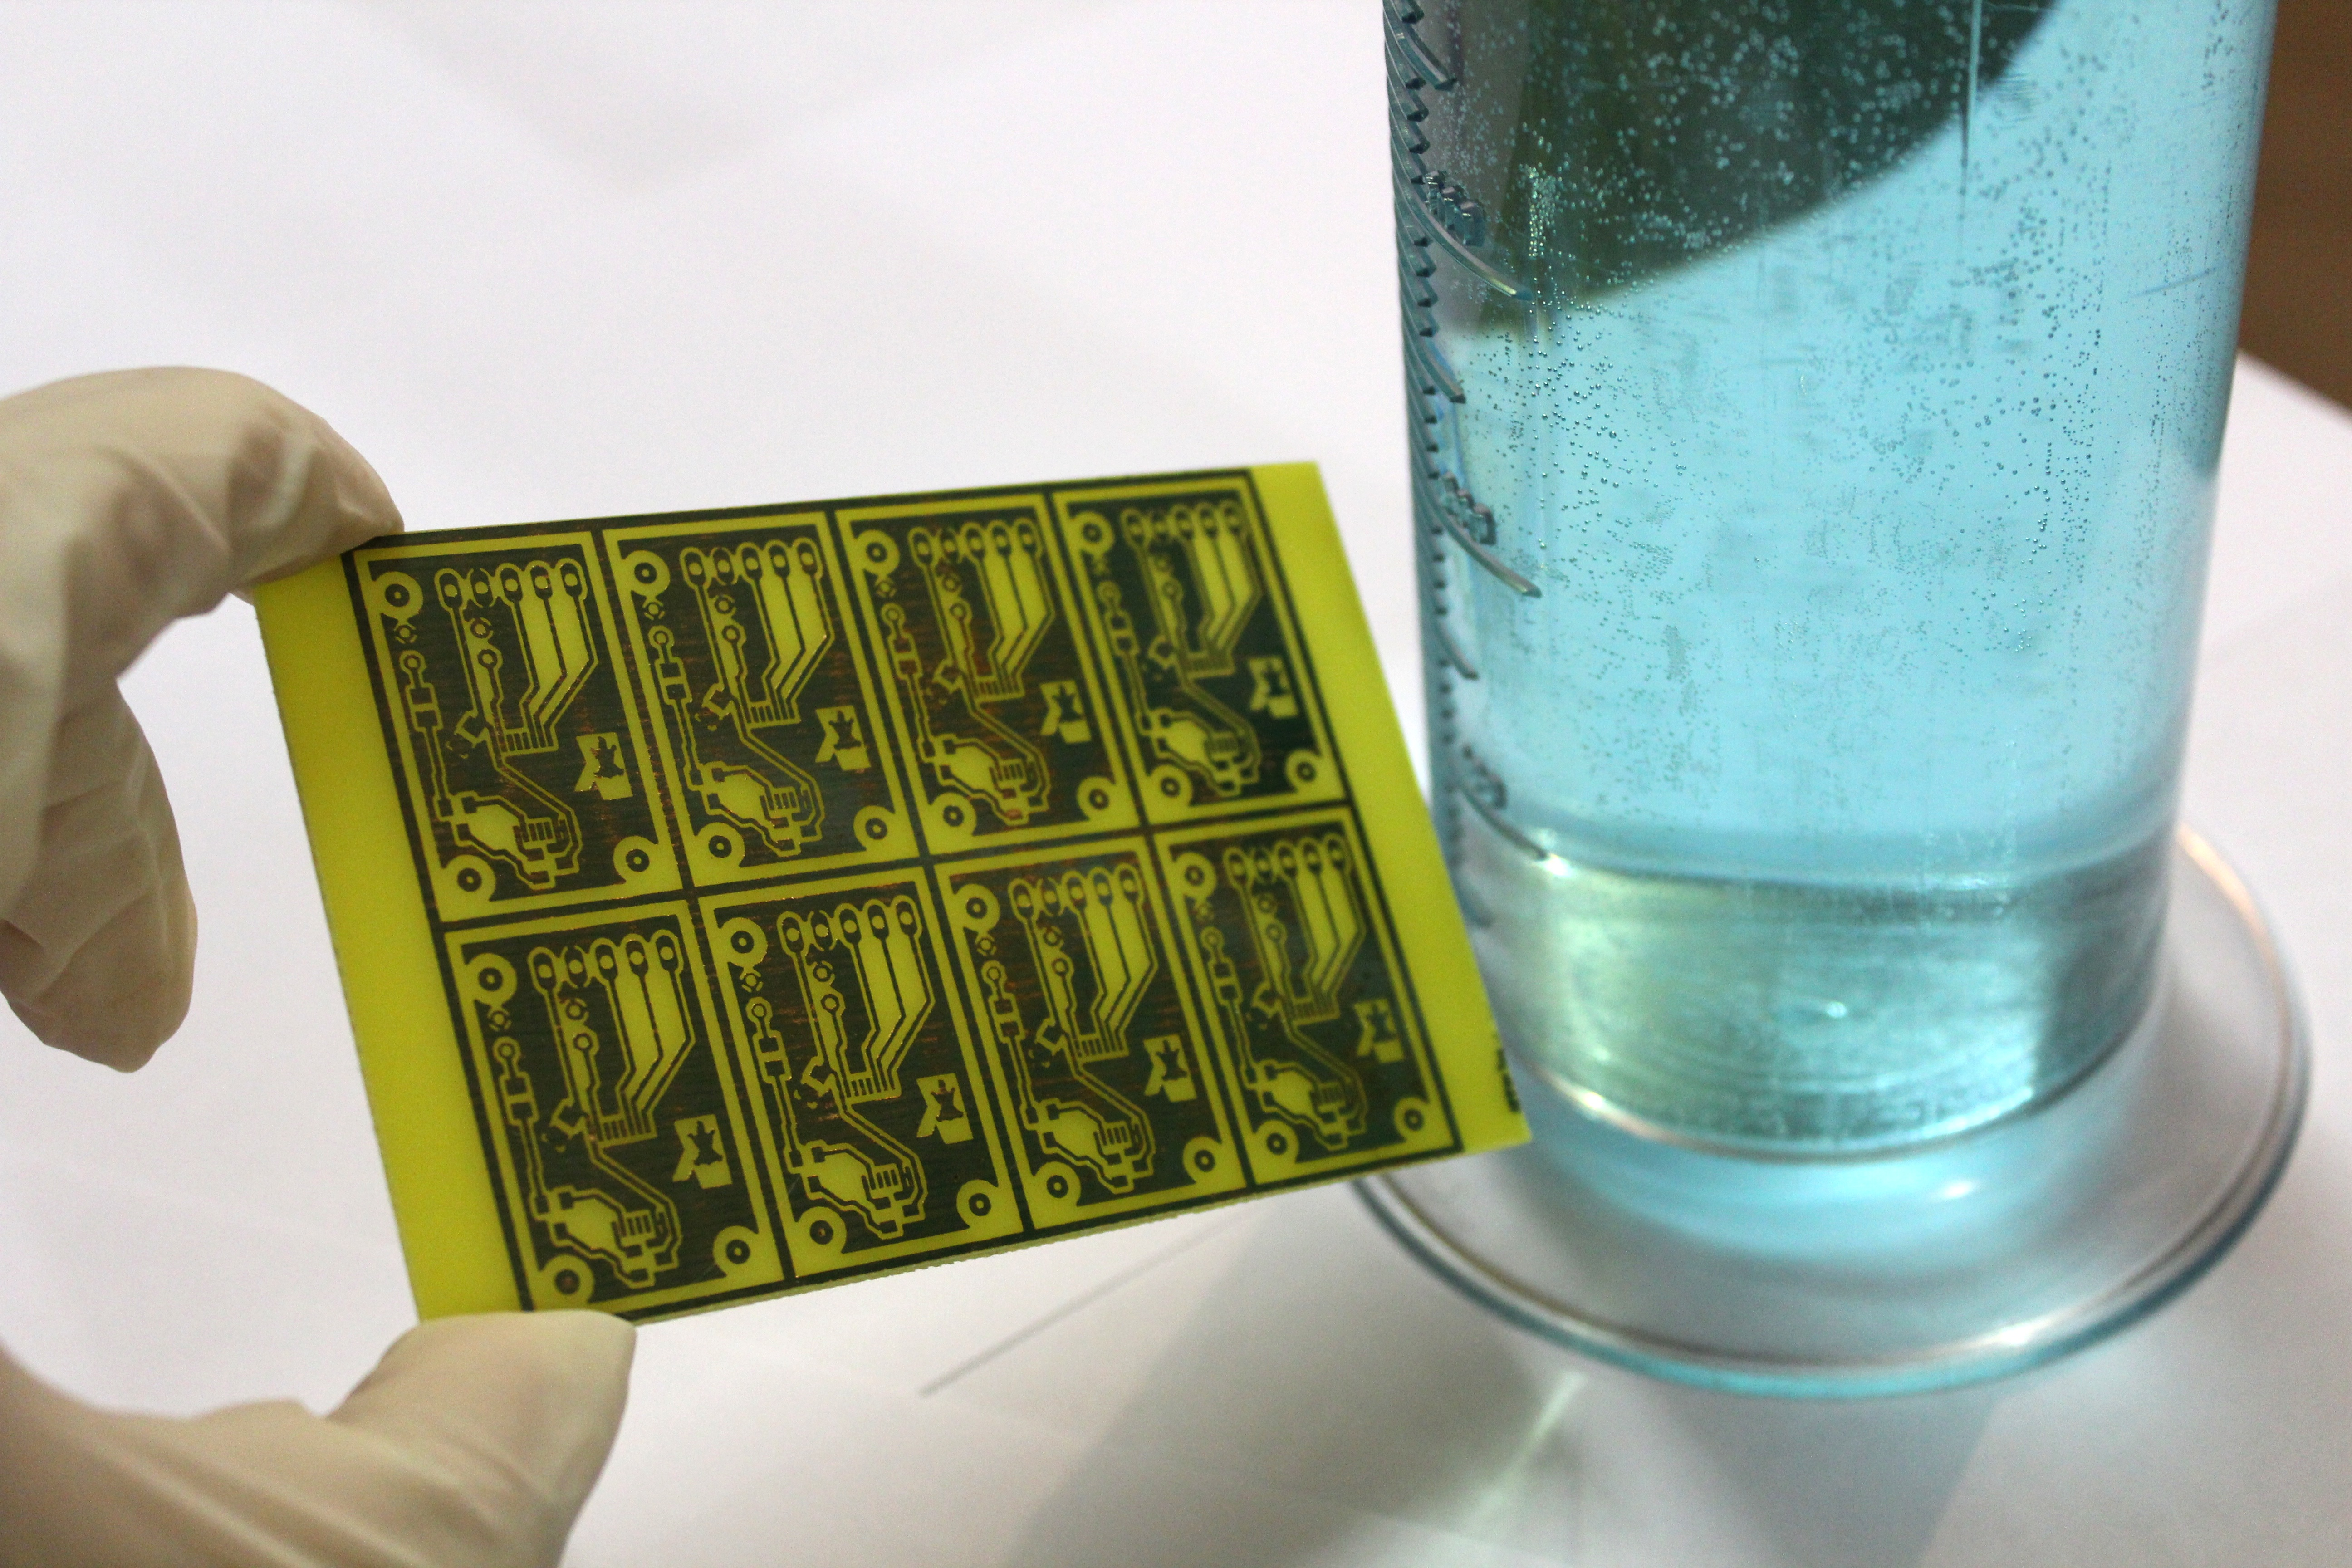
\includegraphics[width=\largeurphoto]{./images/capteurs_apres_gravure.jpg}}\vspace{0.5cm}\\
	\addtolength{\largeurphoto}{\largeurphoto/4}
	\subfloat[La plaque prête à recevoir les composants]{\includegraphics[width=\largeurphoto]{./images/capteurs_pret.jpg}}
\end{figure}

\FloatBarrier

\end{annexe}

\end{annexes}

\end{document}
